\documentclass[]{article}
\usepackage{tikz}
\usepackage{amsmath}
\usepackage{tabto}
\usepackage{fancyhdr}
\usepackage[margin=0.5in]{geometry}
\usetikzlibrary{arrows}
\begin{document}
\begin{center}
\Huge
Recuperacion de Parcial\\
\end{center}
\Large
Problema \# 1\\

\normalsize
\begin{center}
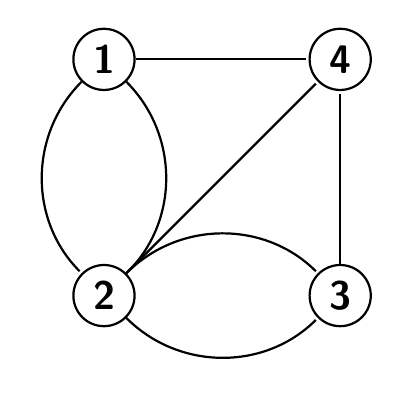
\begin{tikzpicture}[>=stealth',shorten >=1pt,auto,node distance=3cm,
                    thick,main node/.style={circle,draw,font=\sffamily\Large\bfseries}]

  \node[main node] (1) {1};
  \node[main node] (2) [below of=1] {2};
  \node[main node] (3) [right of=2] {3};
  \node[main node] (4) [above of=3] {4};


  \path[every node/.style={font=\sffamily\small}]
    (1) edge[bend left=45] node[above right] {} (2)
		edge[bend right=45] node[above right] {} (2)
		edge node [left] {} (4)
    (2) edge node [left] {} (4)
    	edge[bend right=45] node[above right] {} (3)
    	edge[bend left=45] node[above right] {} (3)
    (3) edge node [left] {} (4);
\end{tikzpicture}\\
Sean las islas los \emph{Nodos} y los puentes los \emph{Vertices}, se obtiene el grafo junto a los conjuntos de nodos y vertices en los cuales el orden de los nodos en el vertice se utiliza simplemente para denotar diferentes formas de llegar al nodo, no indica direccion.\\~\\

\Large
$Nodos = {1,2,3,4}$ \\
\[
Vertices = \begin{bmatrix}
    \langle 1,2 \rangle & \langle 2,1 \rangle & \langle 1,4 \rangle & \langle 2,3 \rangle \\
    \langle 3,2 \rangle & \langle 3,4 \rangle & \langle 2,4 \rangle
\end{bmatrix}
\]
\end{center}
\Large
Problema \# 2\\
\normalsize
\begin{center}

Demostrar por induccion que la siguiente expresion es correcta: $$\sum_{i=1}^{n} i = \frac{n(n+1)}{2}$$\\
Donde $\sum_{i=1}^{n} i = 1+2+3+4+ \ldots +n$\\~\\
Demostrando que para nuestro caso base $i=1$ esta expresion es correcta: $\sum_{i=1}^{n} i = \frac{n(n+1)}{2} = \frac{1(1+1)}{2} = 1$\\~\\
Entonces procedemos a utilizar nuestra suposicion: $\sum_{i=1}^{n+1} i = \frac{n+1((n+1)+1)}{2}$\\~\\
Asumiendo que $\sum_{i=1}^{n} i = 1+2+3+4+ \ldots +n = \sum_{i=1}^{n} i = \frac{n(n+1)}{2}$\\~\\
Entonces $\sum_{i=1}^{n} i = 1+2+3+4+ \ldots +n+(n+1) = \sum_{i=1}^{n} i = \frac{n(n+1)}{2}+(n+1)$\\~\\
$= \frac{n(n+1)}{2}+\frac{2(n+1)}{2}$\\~\\
$= \frac{n(n+1)+2(n+1)}{2}$\\~\\
$= \frac{n+1((n+1)+1)}{2}$\\~\\
\end{center}
\newpage
\Large
Problema \# 3\\
\normalsize
Utilizando la definicion de $\geq$ dada en el \emph{Problema \# 5} y la suma dada en este problema podemos definir la sumatoria de todos los numeros hasta \emph{n} de la siguiente forma:\\~\\
\[
        \sum_{}^{} n =
                \left\{
                        \begin{array}{ll}
                                n = n  & \mbox{si } a = 0$ y $b = 0\\
                                a = a \oplus s(b)$ y $b = b \oplus s(o) & \mbox{si } n \geq s(b) \\
                                \sum_{}^{}n = a & \mbox{si } s(b) \geq n\\
                        \end{array}
                \right.
\]
\Large
Problema \# 4\\
\normalsize
Para demostrar la conmutatividad de la suma. Demostramos el caso base:\\
\begin{center}
Demostramos que,$P(0): a + b = b + a$\\~\\
$P(0): 0 + b = b, b + 0 = b$\\~\\
Ahora, por induccion suponemos que $(a): a + b = b + a$\\~\\
Por induccion llegamos a: $P(s(a)): s(a) + b = b + s(a)$\\~\\
Modificando el lado derecho: $b + s(a)= s(b + a)= s(a + b)$\\~\\
Ya que conocemos la definicion de la suma de numeros naturales unarios, se obvia su demostracion y terminamos con el siguiente resultado:\\~\\
$s(a + b)= s(a) + b$\\
\end{center}
\Large
Problema \# 5\\~\\
\normalsize
Dada la definicion de $a \geq b$\\
\begin{center}
Sabiendo las propiedades de la suma dadas anteriormente en el Parcial, podemos decir que:\\~\\
$(n \oplus n \geq n) = s(o) \rightarrow s(i \oplus n) \geq n = s(o)$\\~\\
Entonces por la definicion de $\geq$ decimos que $i \oplus n \geq i = s(o)$\\~\\
Continuamos con este proceso hasta que $i \oplus n \geq o = s(o)$
\end{center}
\end{document}
